	\subsection{Système de recommandation}	 \label{recommandation}
Dans notre problématique, un système de recommandation pourrait servir à sélectionner les paramètres de jeux, voire le jeu lui même, qui correspondraient le mieux aux besoins du joueur.

\paragraph{}
Les systèmes de recommandation représentent les préférences de l'utilisateur dans le but de proposer des articles à acheter ou à examiner notamment.\\
Rappelons que les besoins du joueur peuvent être soit explicites, notamment à travers les recommandations et exigences du thérapeute, soit plus inconscients. Ces besoins inconscients représentent pas exemple les préférences du joueur-patient en terme de gameplay. Un jeu plus distrayant et motivant pour le patient renforcera son implication dans le programme de réhabilitation, et donc son rétablissement. Pour cela il faut donc à la fois connaître les préférences du patient, explicites ou `découvertes'  grâce à un système d'apprentissage par exemple, mais aussi s'appuyer sur un certain nombre de théories et connaissances que l'on sait efficaces pour renforcer cette immersion. 	
	 
 \paragraph{}
 La proposition est ici de s'inspirer du monde la musique (ou des livres, des films, ou encore des ventes en ligne) et de son système de recommandation.\\
On pense rapidement à deux types de recommandations. La recommandation sociale, qui consiste par exemple à conseiller à un utilisateur des musiques qu'apprécient des personnes de son réseau, surtout si elles écoutent généralement des musiques identiques. Un autre exemple sur les sites de vente en ligne, où l'on propose à un utilisateur venant d'acheter un objet, une liste de produits ayant été achetés en même temps par d'autres utilisateurs. \\
Le second type de recommandation se base pas non pas sur l'environnement social de l'utilisateur, mais sur le contenu même des objets recommandés. L'idée est alors de chercher à décrire un objet selon certaines caractéristiques, et à faire de même pour les préférences de l'utilisateur. On va ensuite lui conseiller les objets qui semblent être le plus proche des attentes de l'utilisateur en se basant sur ces critères de préférences. 
 
\paragraph{}
Pour Vincent Castaignet\cite{Cast11}, fondateur et directeur de la publication de Musicovery, au-delà de la recommandation éditoriale, il y a différentes manières de proposer des artistes/titres par similarité~:
\begin{enumerate}
	\item d’après les formes musicales sur lesquelles le goût des auditeurs est fondé.
	\item d’après les repères mentaux utilisés par les auditeurs (genres, sous-genres, style).
	\item social  : si tu es membre de cette tribu et aimes cet artiste, alors tu vas aimer ces artistes.
	\item contextuel  : ceux qui écoutent ce titre dans ce contexte écoutent aussi ces titres.
\end{enumerate}
Les passionnés de musique qui cherchent activement préféreront de la similarité type (2), le grand public plus passif de la similarité type (4). Un moteur de similarité intelligent devrait pouvoir combiner ces différentes formes et s’adapter en fonction du profil de chacun.
Pandora est principalement construit sur (1), last.fm est (2) et (3), Musicovery (4). Deezer avec ces 30 millions de playlists a un actif considérable à exploiter en (3) et (4).

 		\subsubsection*{Les différents types de recommandation}
Plusieurs techniques de recommandation ont été proposées\cite{Burk02} : basées sur le contenu, sur des connaissances ou encore des techniques dîtes collaboratives ou sociales. Pour de meilleurs résultats, certaines de ces techniques peuvent être utilisées conjointement dans des systèmes de recommandation hybrides.

	\paragraph{\emph{Propriétés des systèmes de recommandation} \\ \quad}
Les systèmes de recommandation possèdent\cite{Burk02}~:
\begin{itemize}
	\item des données de base : données que le système possède avant même de commencer la recommandation
	\item des données d’entrée : données que l’utilisateur fournit au système dans le but que ce dernier lui fournissent des recommandations.
	\item un algorithme qui utilise ces données de base et d’entrée pour générer les résultats.
\end{itemize}

	\paragraph{}
\begin{figure}[hbtp]
	\centering
	On peut distinguer 5 types de systèmes de recommandation
	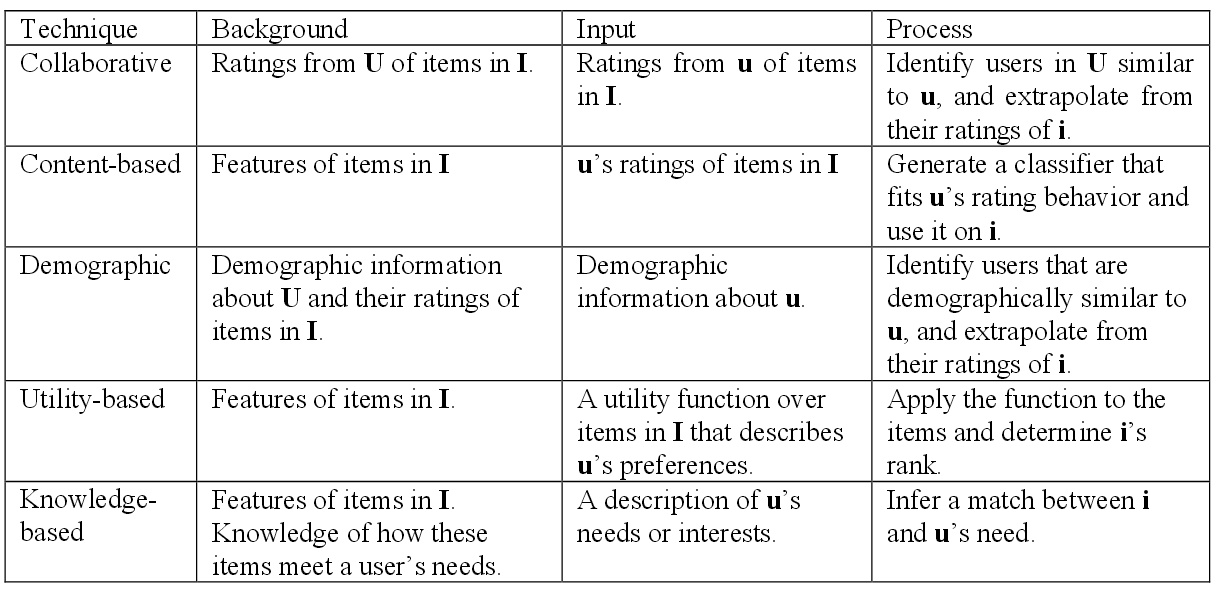
\includegraphics[width=1\linewidth]{images/types_recommandation.png}
	\caption{Techniques de recommandations [R. Burke, 2002] \cite{Burk02} }
	\label{types_recommandation}
\end{figure}    
avec :
\begin{itemize}
	\item I : ensemble d’objets sur lequel sont faites les recommandations
	\item U : l’ensemble d’utilisateurs dont les préférences sont connues
	\item u : l’utilisateur pour lequel les recommandations doivent être générées
	\item i : objets pour lesquels on souhaiterait prédire une préférence de la part de u
\end{itemize} 

		\paragraph{\emph{Collaborative} \\ \quad}
Méthode la plus mature et répandue. Le système agrège les notes ou recommandations des objets, relève les similarités entre les appréciations des utilisateurs et en déduit de nouvelles recommandations pour les utilisateurs. Certains systèmes prennent le temps en paramètre dans leur évaluation afin de prendre en compte l’évolution de l’intérêt des utilisateurs au fil du temps (effet de mode, etc). L’évaluation peut être simplement binaire ou plus complexe en utilisant une échelle de graduation. Les systèmes peuvent être soit basés sur une mémoire, comparant les utilisateurs par corrélation ou autre, soit basés sur un modèle :  celui-ci est dérivé à partir de l'historique des données d'évaluation et utilisé pour faire les prédictions.
La plus grande force de ces techniques est qu’elles sont complètement indépendantes de la représentation informatique des objets recommandés.

		\paragraph{\emph{Démographique} \\ \quad}
Ces systèmes de recommandation ont pour but de catégoriser l’utilisateur à partir de ses caractéristiques propres et de faire des recommandations en fonction de son appartenance à l’une des classes démographiques prédéfinies. L’avantage d’une approche démographique est qu’elle ne requiert pas un historique des évaluations des utilisateurs à l’inverse des méthodes collaboratives et basées sur le contenu.

		\paragraph{\emph{Basée sur le contenu} \\ \quad}
 La recommandation basée sur le contenu est une excroissance et la poursuite de la recherche d'information de filtrage. Dans ces systèmes, les objets sont définis en fonction de leurs caractéristiques associées. Le système apprend à connaître le profil de l’utilisateur en se basant sur les caractéristiques des objets évalués par l’utilisateur. C’est une corrélation objet-à-objet. Le profil dérivé dépend évidemment du type d’apprentissage employé : arbre de décisions, réseaux de neurones et représentations par vecteurs sont utilisés.

		\paragraph{\emph{Fondée sur l’utilité} \\ \quad}
Ces systèmes font des suggestions en se basant sur une estimation de l’utilité de chaque objet pour l’utilisateur. Le problème central étant comment créer cette fonction d’utilité pour chaque utilisateur. D’abord évaluer les objets (différentes méthodes), puis le profil utilisateur, avant de calculer la correspondance entre les deux. L’avantage de la technique est qu’elle peut prendre en compte des attributs non directement propres aux objets évalués (fiabilité du vendeur, disponibilité du produit, etc.) pour proposer des recommandations plus pertinentes (besoin immédiat ou meilleur prix par ex.).

		\paragraph{\emph{Basée sur le savoir/connaissance} \\ \quad}
Tenter de recommander des objets en inférant les besoins et préférences de l’utilisateur. Ces systèmes se distinguent en ce qu’ils ont un savoir fonctionnel : ils ont connaissance que tel objet répond à tel besoin et peuvent alors abstraire la relation entre le besoin et une possible recommandation.

	\paragraph{}
Les systèmes de recommandations basés sur l’utilité et sur le savoir n’essaient pas de construire des généralisations à long terme à propos de leurs utilisateurs, mais préfèrent baser leurs conseils sur une évaluation de la correspondance entre les besoins d’un utilisateur et un ensemble d’options disponibles.
